\clearpage
\subsection{Original source: partial gas exchange at saved ceramic fields}
A source-only subset pairs bare ceramic surface patches through vertical columns that avoid the source solid bounding volumes. The three paired unblocked areas are 7.428, 5.498 and 1.979 mm$^2$. They are disjoint surface allocations, not a complete gas-domain solution or bounds on total physical gas heat flow. The annular enclosure is excluded from the blocking test only where its inner radius is demonstrably outside the working footprint.

For 100 Pa krypton, applying a Maxwell-type temperature-jump conductance to these 752 cells and sampling the archived four ceramic temperature fields gives the following hot-to-cold heat flows. The gas accommodation coefficient $\alpha$ is an assumed sensitivity, not a measured material property.
\begin{center}\small\begin{tabular}{lrrr}\toprule
$\alpha$ & C0--C1 (mW) & C1--C2 (mW) & C2--C3 (mW) \\ \midrule
0.5 & 1.900574 & 0.918993 & 0.401021 \\
0.8 & 2.519773 & 1.188742 & 0.506549 \\
1.0 & 2.826754 & 1.317665 & 0.555253 \\
\bottomrule\end{tabular}\end{center}
Each link applies equal and opposite heat to its two ceramics; the four resulting loads sum to zero. Node temperatures are nearest-source-node samples, with maximum lateral distance 0.1784 mm. The calculation is one-way: the old ceramic fields are held fixed, other gas surfaces are omitted for this diagnostic, and no new detector temperature is predicted. A physically coupled calculation still requires conservative subface integration and allocation of all other gas-facing surfaces; gas diffusion across the connected cavity is not represented by independent columns.

The eight lead-joint gas faces now have source-backed wire and pad or pin contact identities and provisional endpoint temperatures. The patterned-metal and P/N side temperatures remain approximations, the full metal-field electrical gate remains failed, and no native gas boundary condition has been qualified.
\begin{figure}[htbp]\centering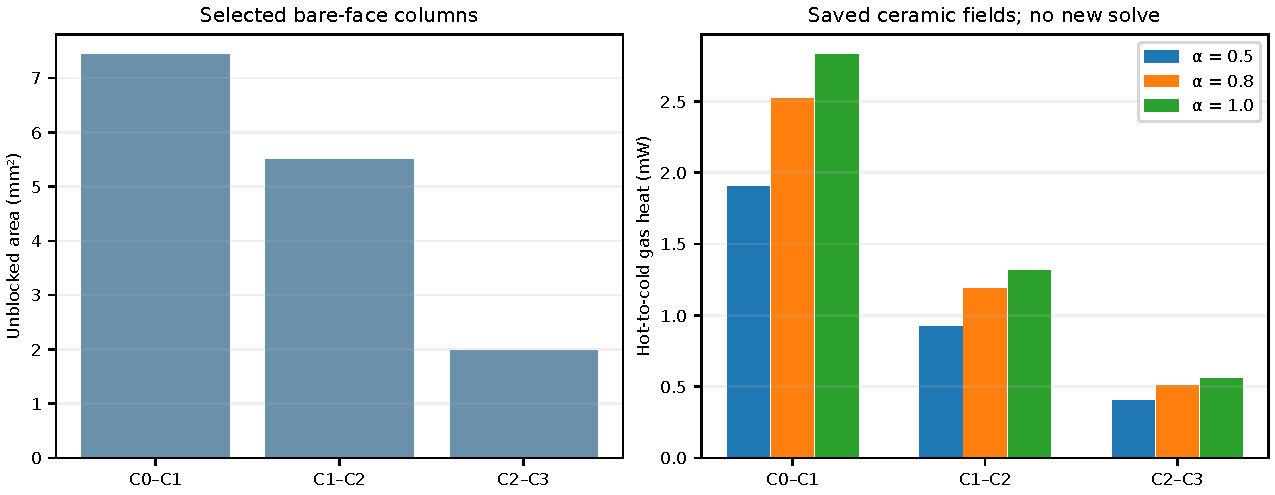
\includegraphics[width=.96\linewidth]{figures/v324_nominal_gas_subset.pdf}\caption{Original-source subset areas and gas-link calculations at archived ceramic fields. The three accommodation settings are hypotheses; omitted cavity paths and the absence of a new coupled solve preclude interpreting the bars as total package gas heat.}\end{figure}
